%%%%%%%%%%%%%%%%%%%%%%%%%%%%%% -*- Mode: Latex -*- %%%%%%%%%%%%%%%%%%%%%%%%%%%%

%% textemplate.tex -- IEEE Software Paper on Telemetry

%% Author          : Philip Johnson

%% Created On      : Mon Sep 23 11:52:28 2002

%% Last Modified By: Philip Johnson
%% Last Modified On: Fri Sep 24 16:19:37 2004
%% RCS: $Id$

%%%%%%%%%%%%%%%%%%%%%%%%%%%%%%%%%%%%%%%%%%%%%%%%%%%%%%%%%%%%%%%%%%%%%%%%%%%%%%%

%%   Copyright (C) 2002 Philip Johnson

%%%%%%%%%%%%%%%%%%%%%%%%%%%%%%%%%%%%%%%%%%%%%%%%%%%%%%%%%%%%%%%%%%%%%%%%%%%%%%%

%% 



%% This is a sample file showing how to produce CSDL TechReports in ICSE

%% conference style using LaTeX.  It can be adapted to thesis structure

%% with very minor changes. 





\documentclass[11pt,twocolumn]{article} 

\input{/export/home/csdl/tex/psfig/psfig}

\usepackage{/export/home/csdl/tex/icse2003/latex8}

\usepackage{times}

%% A verbatim-like environment which allows font changes

%%\usepackage{alltt}

%% New LaTeX2e graphics support

\usepackage[final]{graphicx}

% uncomment the % away on next line to produce the final camera-ready version

% and uncomment the \thispagestyle{empty} following \maketitle

\pagestyle{empty}



\begin{document}



\title{Improving Software Development Management \\ through Software Project Telemetry}





\author{\protect\begin{tabular}{ccc}

Philip M. Johnson & Hongbing Kou & Michael Paulding  \\

Qin Zhang & Aaron Kagawa & Takuya Yamashita \\

\end{tabular}\\

\em  Collaborative Software Development Laboratory \\

\em  Department of Information and Computer Sciences \\

\em  University of Hawai'i \\

\em  Honolulu, HI 96822 \\

\em  johnson@hawaii.edu}

\maketitle

\thispagestyle{empty}



\begin{abstract}  % 200 words



foo
Software project telemetry is a new approach to software project

management in which sensors are attached to development environment tools

to unobtrusively monitor the process and products of development. This

sensor data is abstracted into high-level perspectives on development

trends called Telemetry Reports, which provide project members with 

insights useful for local, in-process decision making.  This paper presents

the essential characteristics of software project telemetry, contrasts it

to other approaches such as predictive models based upon historical

software project data, describes a reference framework implementation of

software project telemetry called Hackystat, and presents our lessons

learned so far. 



\end{abstract}



\Section{Introduction}

\label{sec:intro}



It is conventional wisdom in the software engineering research community

that metrics can improve the effectiveness of project management.

Proponents of software metrics quote theorists and practitioners from

Galileo's ``What is not measurable, make measurable'' \cite{Finkelstein82}

to DeMarco's ``You can neither predict nor control what you cannot

measure'' \cite{DeMarco82}.  Software metrics range from internal product

attributes, such as size, complexity, and modularity, to external process

attributes, such as effort, productivity, testing quality, and reliability

\cite{Fenton97}. 





\begin{figure*}[ht]

  \centering

  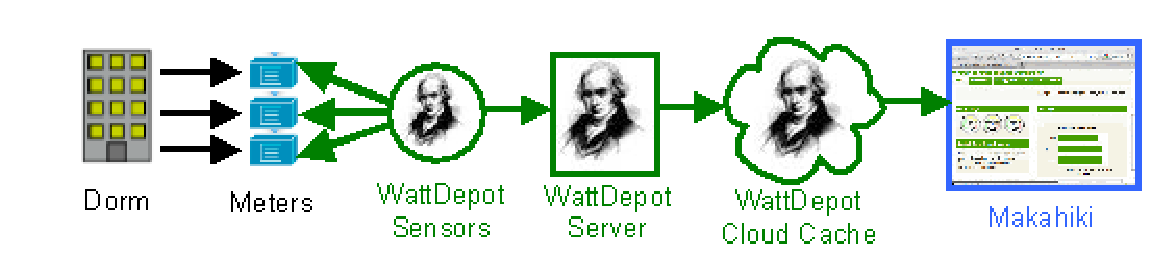
\includegraphics[width=0.75\textwidth]{architecture.eps}

  \caption{The basic architecture of Hackystat. Sensors are attached to

  tools directly invoked by developers (such as Eclipse or Emacs) as

  well as to tools implicitly manipulated by developers (such as CVS or 

  an automated build process using Ant).}

  \label{fig:architecture}

\end{figure*}





\bibliographystyle{/export/home/csdl/tex/icse2003/latex8}

\bibliography{/export/home/csdl/techreports/04-11/04-11,/export/home/csdl/bib/csdl-trs,/export/home/csdl/bib/hackystat,/export/home/csdl/bib/psp}

\end{document}

 





















